% Figure / table inputs

\chapter{Approach and Custom Software solutions} \label{chap:3}
\todo[inline]{replace CITEME tags in Approach and Custom Software solutions}


Frequently, \gls{functional-genomics} approaches contain problems or subproblems that require generating biologically meaningful gene-sets that pertain to the focus of the particular phenomenon being targeted.
Optimizing signal-to-noise ratios in data is a major challenge to generating useful gene-sets.
This project aims to generate meaningful gene-sets through integrating information from four supporting data-types:

\begin{itemize}
    \item comparative genomics ($N$-way 1-to-1 ortholog relationships)
    \item comparative transcriptomics (identical RNA-seq experiments performed using divergent mosquito species with the shared trait of \gls{hematophagy})
    \item phylogenetics (estimated divergence since last common ancestor)
    \item putative regulatory mechanisms (predicted \gls{TFBS} profiles)
\end{itemize}



\section{Approach}

\paragraph*{Comparative Genomics:}

The initial gene-set for this project was limited to genes that have exactly one matching 1-to-1 ortholog in \Aa, \Ag, \As, and \Cq.
The purpose of this constraint is to maximize the probability of conserved function between genes analyzed. 

This preliminary gene set was obtained using the orthoDB7 \url{http://cegg.unige.ch/orthodb7} website by first selecting the node representing only the mosquito branch of the phylogeny \cite{Waterhouse2013}.
Then, the following requirements were enforced when retrieving ortholog relationship results 

\begin{quotation}
    \texttt{co-ortholog copy-number: AAEGY=1, AGAMB=1, ASTEP=1, CQUIN=1}
\end{quotation}


\begin{landscape}

\begin{figure}[hp]
\centering
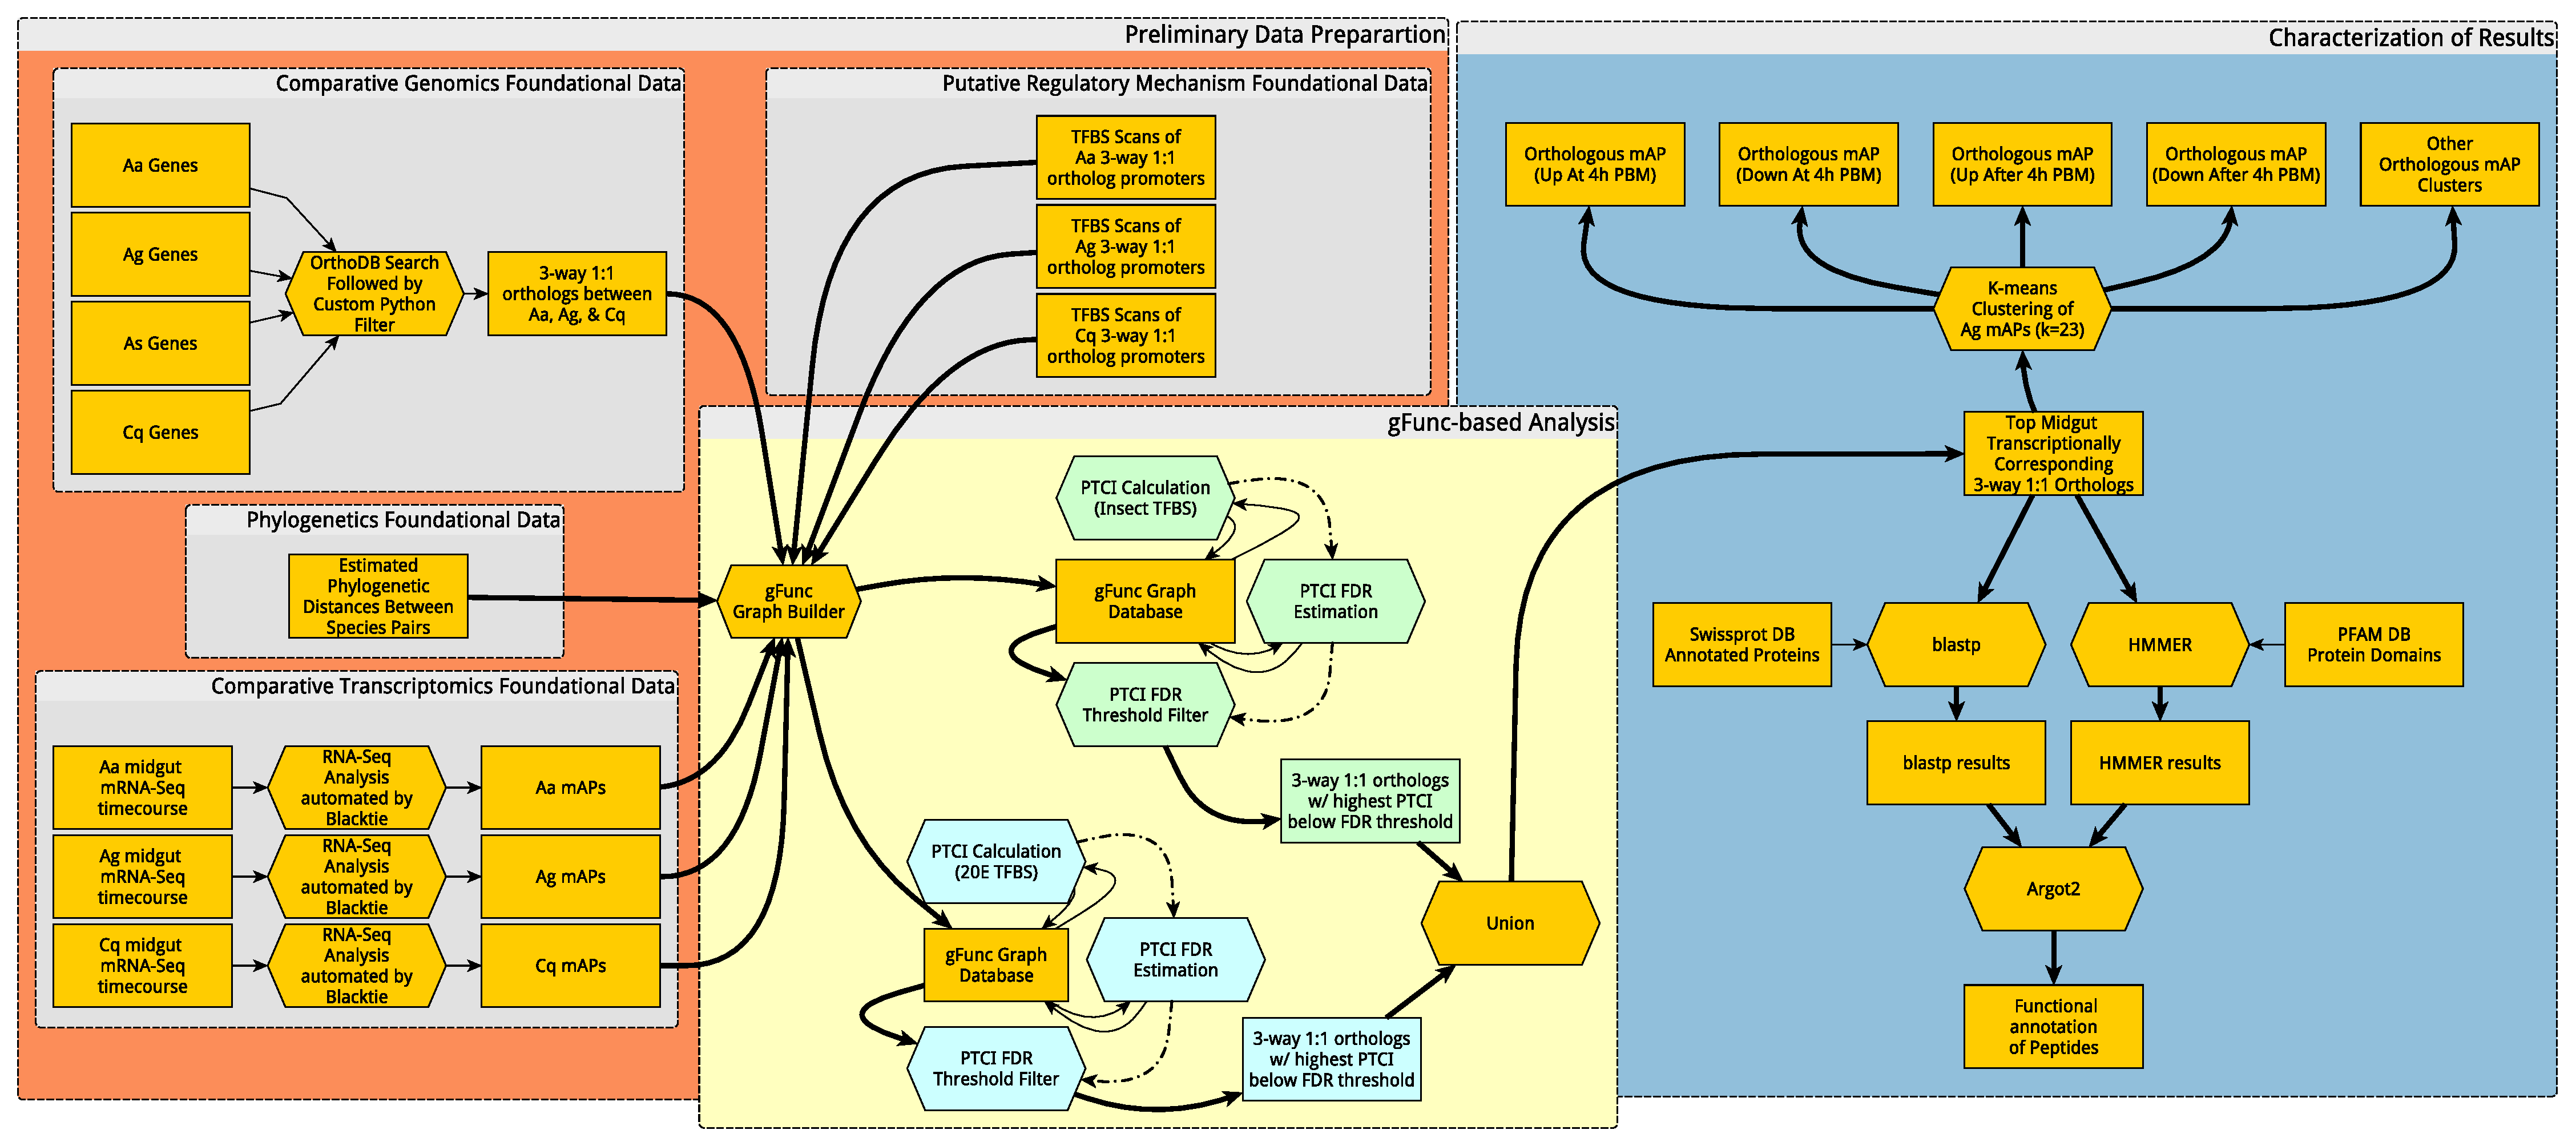
\includegraphics[width=\linewidth]{figures/figs/approach_chart/approach_overview.pdf}

\caption[Input-output diagram of approach overview]{
\sf \textbf{Input-output diagram of approach overview:}
%
The approach employed can be divided into three stages.
\emph{Preliminary Data Preparation }consists of accumulating and preparing the foundational data representing the four data-types to be integrated into the \gls{gFunc} graph.
\emph{gFunc-based Analysis} involves mapping the foundational data onto the gFunc graph structure and submitting the graph to custom Python functions that read, analyze, and write results back to the graph to calculate the \glspl{PTCI} and corresponding \glspl{FDR}.
This is done using two \gls{TFBS} profile data-sets with results being merged by a union-type set-operation to obtain the overall set orthologs representing putatively conserved midgut \glspl{mAP}.
\emph{Characterization of Results} then uses \gls{Argot2} \cite{Falda2012} to obtain functional annotations of the ortholog-sets, and the \glspl{mAP} of \Ag\ members are clustered using k-means clustering to group the ortholog-sets by expression similarity.


\emph{Heavy Arrows:} main flow of data;
\emph{Light Arrows:} preliminary or minor data flow;
\emph{Dashed Arrows:} establishes the order of execution;
\emph{Square Node:} data set;
\emph{Hexagon Node:} analysis operation.

}
\label{fig:approach-chart}
\end{figure}

\end{landscape}

The results of the query are provided as file \texttt{orthodb7\_mosqs\_20130918.txt} in the supplementary data files associated with this dissertation \cite{Dunn2013dissSupl}.
 
Custom python code was used to extract the 1-to-1 orthologs for \Aa, \Ag, and \Cq\ (Figure \ref{fig:approach-chart}).
The coded process is provided as an executable IPython notebook located at \url{http://goo.gl/EM1pHL} for in-depth inspection as well as for the purpose of openness and reproducibility.

Briefly, the results table was filtered for data pertaining to \Aa, \Ag, or \Cq.
Then I built a graph-representation of the data such that each orthoDB ortholog group could be queried to ensure that exactly one gene was represented for each species of interest.
These genes represent gene-set that formed the starting point for the rest of my approach.
The filtered set is available as supplementary file \texttt{AaAgCq\_1to1\_orthos.tsv} \cite{Dunn2013dissSupl}.

It should be noted that while this set contains only genes from the three species included in this document, each group should also have exactly one ortholog from \As\ as well which represents an additional constraint intended to limit the ortholog-sets to those most likely to fulfill the same function in each species.

\paragraph*{Comparative Transcriptomics:}

Whole RNA was extracted from dissected midguts of 16 female individuals of each species among the following time points: \gls{NBF} (0), 2, 4, 6, 8, 10 h \gls{PBM} (Protocol \ref{prot:RNA_Judy}) to identify and analyze orthologous genes that exhibit correlated \glspl{mAP} in the midguts of females directly following the ingestion of a bloodmeal.


\paragraph*{Phylogenetics:}

The phylogenetics aspect of this approach consists of using the estimated phylogenetic distances between each species to weight the comparisons between data correlations calculated for each pairwise 1-to-1 ortholog duo.
This is encoded as $d$ in the \gls{PTCI} expression defined in Equation \ref{eq:ptci} (see Section \ref{sec:ptci}).

The values of $d$ for each species-pair have been estimated previously (Table \ref{tab:evo-ranges}) (compiled in \citet{Sieglaff2009}).


\begin{table}[h]
\centering \sffamily
{%
\newcommand{\mc}[3]{\multicolumn{#1}{#2}{#3}}
\begin{center}
\begin{tabular}{llc}\toprule
\mc{2}{c}{\textbf{Species Pair}} & \textbf{Mya}\\ 
\midrule
\Aa & \Ag & 145\\
\Ag & \Cq & 145\\
\Aa & \Cq & 22\\ \bottomrule
    \end{tabular}
    \end{center}
}%

\caption[Estimated pairwise-evolutionary divergence between species]{\bsf{Estimated pairwise-evolutionary divergence between species}}
\label{tab:evo-ranges}
\end{table} 



% 
%     \Aa \Ag = 145 MYA 
%     \Ag \Cq = 145 MYA 
%     \Aa \Cq = 22 MYA  
%     




\paragraph*{Putative Transcriptional Regulatory Control Mechanisms:}

Part of the \gls{PTCI} includes correlation of a \gls{TFBS} scanning signature between ortholog pairs.
If the \gls{PTCI} is calculated using a set of \gls{TFBS} that are known to interact with the \gls{20E} signaling cascade, then this portion of the \gls{PTCI} acts as a rough proxy for correlation with putative activity of the \gls{20E} cascade.

The \gls{TFBS} profiles are obtained through scanning the 2000 bp regions 5' to the annotated start of transcription for each gene using the \gls{MOODS} application wrapped in custom Python code \cite{Pizzi2009}.
The scoring method used was log-odds.
The final \gls{TFBS} profile score for a gene-motif combination consists of the sum of all site-scores with positive log-odds scores.
In this way the gene-motif score represents the count of all site-scores that fit the motif model better than would be expected after considering the background sequence-composition of the putative promoter-regions weighted by the log-odds value of each site-score.
For example, for motif model $m$, if one sequence had three sites that each received log-odds scores of 0.33, then the gene-motif score is approximately 1.
Alternatively, if a second sequence has a single site that matches $m$ with a positive score of 1, both sequences would have approximately equal gene-motif scores for $m$.
Just as the \gls{mAP} for a particular gene consists of 5 values that represent the \gls{FPKM} score for that gene at 5 time-points, the \gls{TFBS} profile of a gene consists of $N$ values (the number of motif models considered) that represent the sum of sites in the putative promoter region that received a positive log-odds value weighted by the log-odds value of each site.

This is an imperfect solution as \gls{ChIP-Seq} using antibodies to specific \glspl{TF} in each species is preferable\footnote{those that are presently associated with \gls{20E} for instance}.
However this was impractical for this work due to the absence of suitable antibodies and the cost of developing and executing all assays in each species.


\section{The phylogenetic transcriptional correspondence index (PTCI)} \label{sec:ptci}

The \gls{PTCI} (Equation \ref{eq:ptci}) attempts to provide a metric that combines multiple pairwise \gls{Pcc} ($r$) relating to multiple comparison dimensions pertaining to each 1:1 ortholog pair and then weight it using the relative evolutionary divergence times of each pairwise comparison ($d$).
%


\begin{equation} \label{eq:ptci}
PTCI = ( r_{x} + \frac{r_{t}}{2} ) \cdot w(d)
\end{equation}

%
In Equation \ref{eq:ptci}, the two comparison dimensions being combined are the similarity between an ortholog-pair with respect to \gls{mAP} ($r_{x}$) and \gls{TFBS} profile signature ($r_{t}$).
The pairwise species-divergence is represented by $d$.
However, the divergence times must be transformed using a scaling function ($w()$) that prevents the \textbf{much} larger values of raw divergence values from dominating the index.
I have chosen to constrain the range of $w(d)$ between $1$ (no reward) and $1.1$ (a reward of 10\%).
This range was chosen to allow the evolutionary distance to affect the ranking of an ortholog-set without having a dominating effect.
I explored other settings, but this range appeared to be a good compromise (not shown).
%




\begin{figure}[hp]
\centering
  \begin{subfigure}[b]{.9\linewidth}
    \centering

    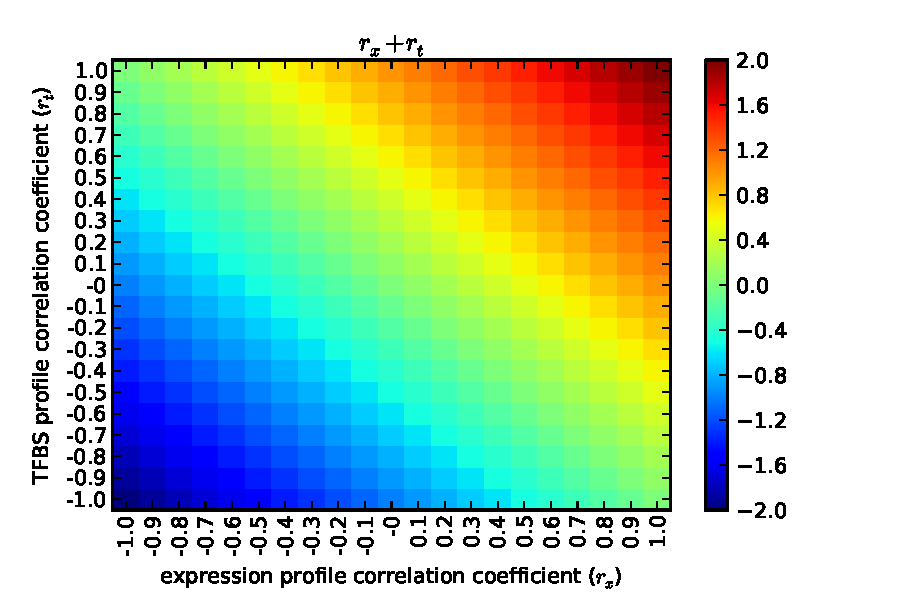
\includegraphics[width=.9\linewidth]{figures/figs/thesis-xprn-tfbs.pdf}
    \caption{}
    \label{fig:ptci-space-a}
  \end{subfigure}%

  

  \begin{subfigure}[b]{.9\linewidth}
    \centering

    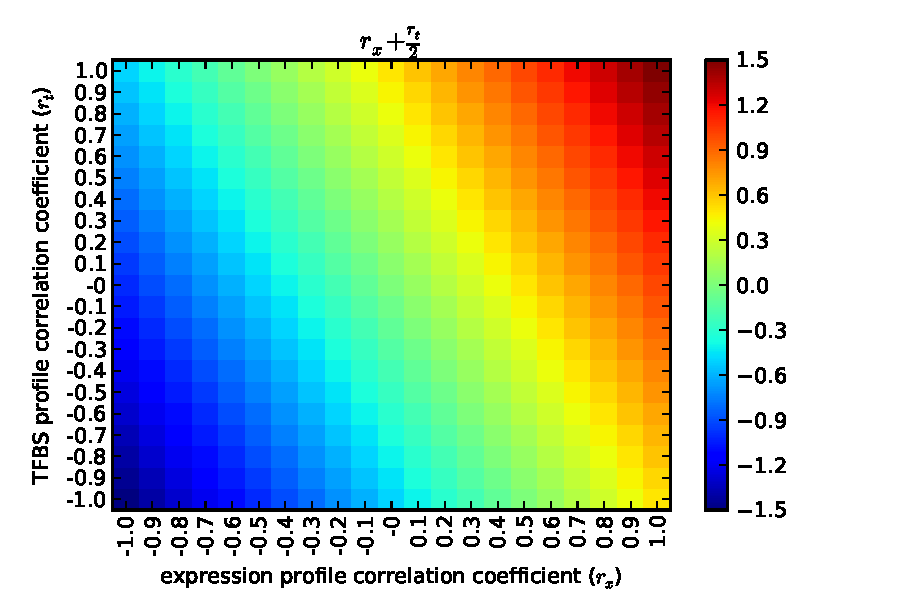
\includegraphics[width=.9\linewidth]{figures/figs/thesis-xprn-scaled-tfbs.pdf}
    \caption{}
    \label{fig:ptci-space-b}
  \end{subfigure}

\caption[Exploring the parameter space of the expression and TFBS components of the PTCI]{\sf \textbf{Exploring the parameter space of the expression and TFBS components of the PTCI:} \\
\textbf{(A)} The expression and TFBS profile correlations each carry the same weight.  TFBS data is not strictly empirical, and position weight matrix models inherently are prone to produce false positive predictions. Here, each correlation-type exerts equal influence on the final score assigned to the ortholog relationship.  \textbf{(B)} The TFBS profile correlation is penalized due to the non-empirical nature and expected false positive information it contains. Here, TFBS profile data contributes to the final score at most 50\% as much as expression data.}
\label{fig:ptci-space}
\end{figure}
%
The \gls{TFBS} data is derived through imperfect and non-empirical means.


(Figure \ref{fig:ptci-space}).





The graph model is useful (Figure \ref{fig:nway-ortholog-graph})


\begin{figure}[hp]
\centering
% 
    \begin{subfigure}[t]{.5\linewidth}
    \centering
    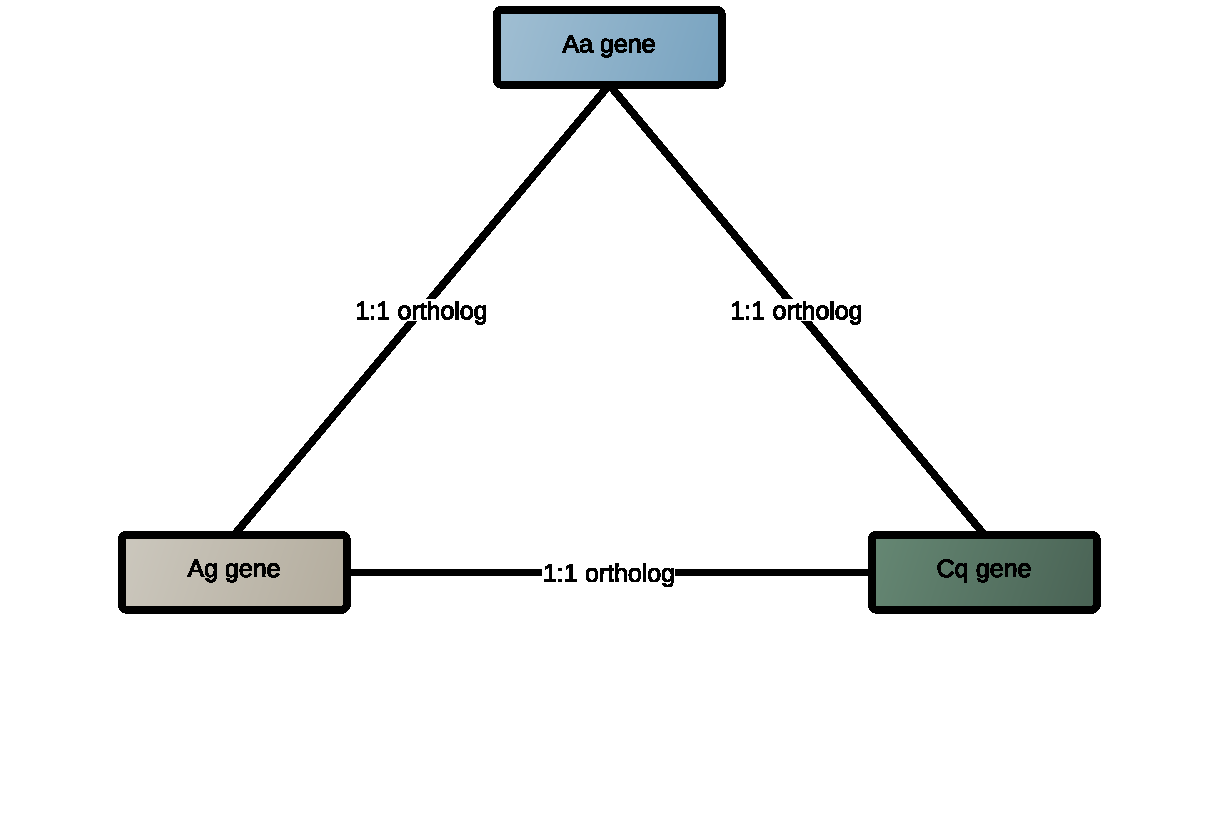
\includegraphics[width=\linewidth]{figures/figs/gfunc_graph_figs/ortho-graph-model.pdf}
    \caption{N-way 1:1 ortholog graph structure}\label{fig:nway-ortholog-graph-model}
    \end{subfigure}%
% 
% 
% 
    \begin{subfigure}[t]{.5\linewidth}
    \centering
    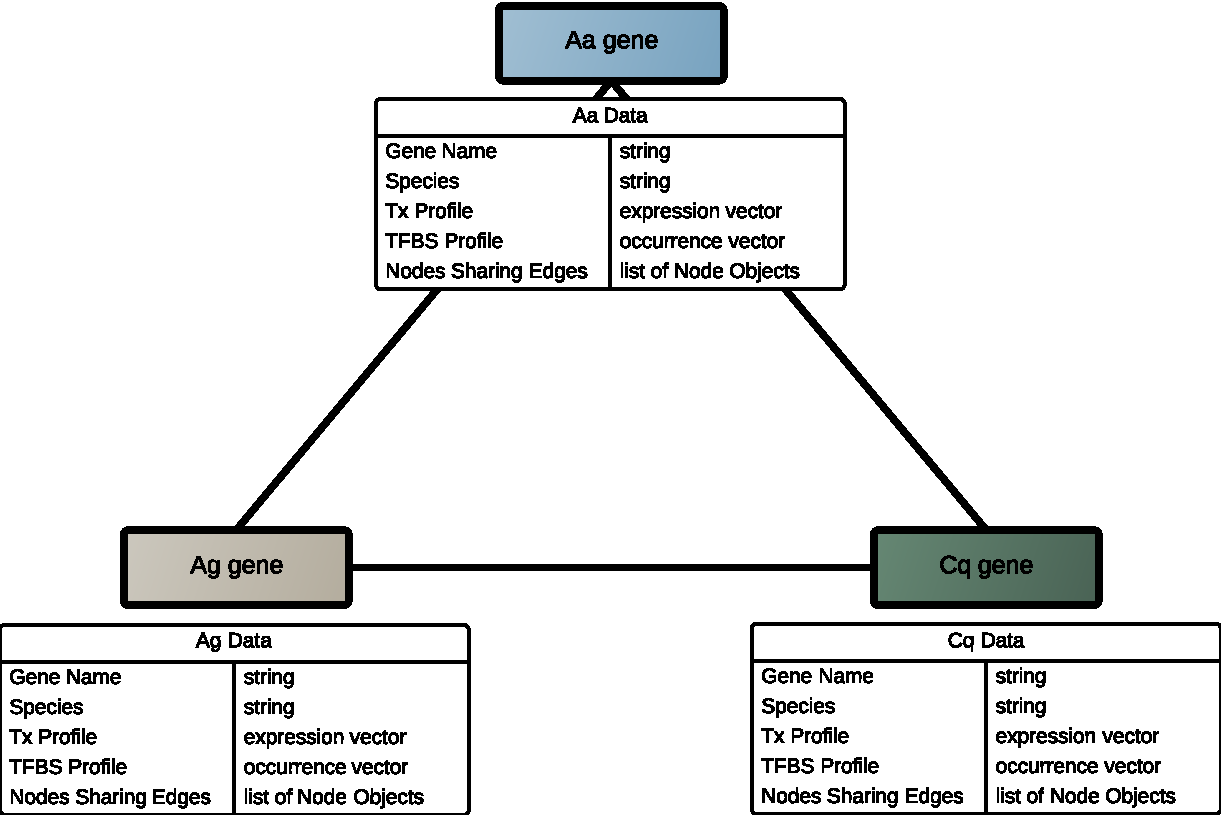
\includegraphics[width=\linewidth]{figures/figs/gfunc_graph_figs/ortho-graph-node-data.pdf}
    \caption{Node data model}\label{fig:nway-ortholog-graph-node-data}
    \end{subfigure}
% 
% 
% 
% 
% 
% 
    \begin{subfigure}[t]{.5\linewidth}
    \centering
    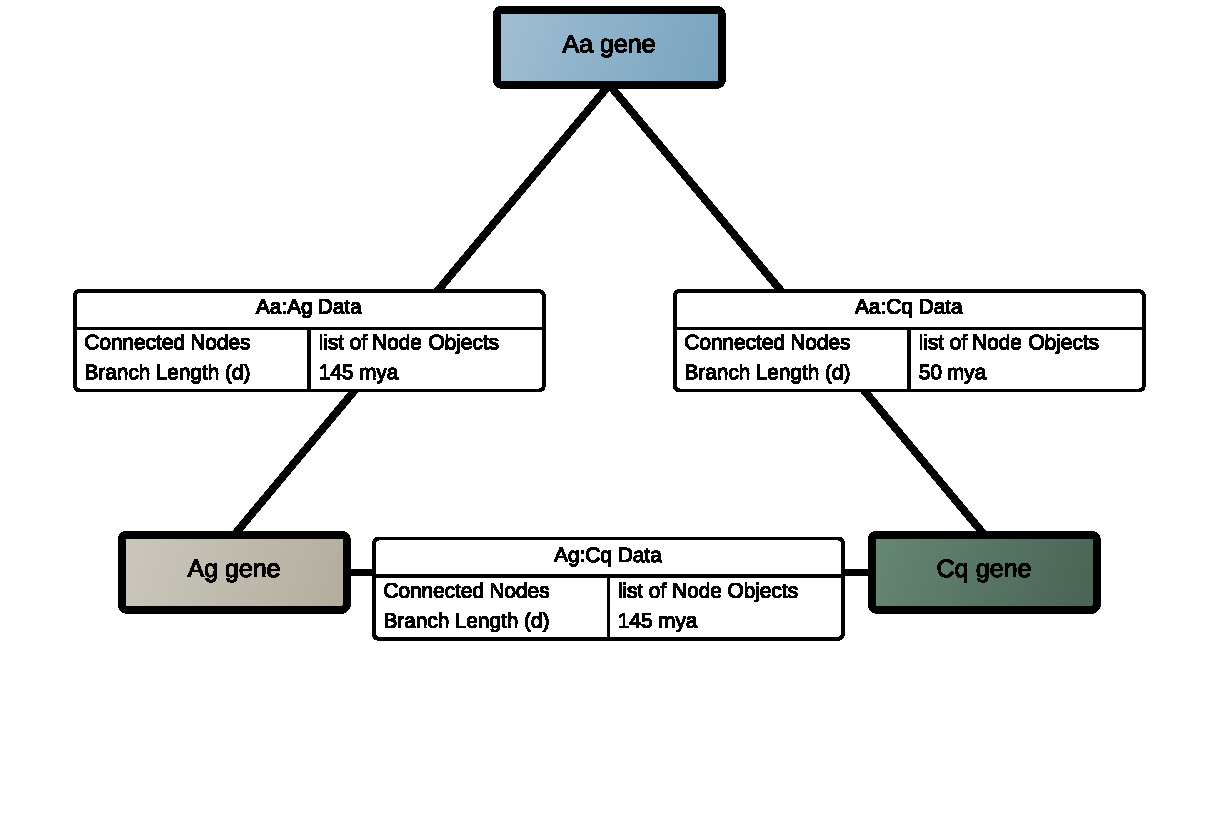
\includegraphics[width=\linewidth]{figures/figs/gfunc_graph_figs/ortho-graph-edge-data.pdf}
    \caption{Edge data model}\label{fig:nway-ortholog-graph-edge-data}
    \end{subfigure}%
% 
% 
%     
    \begin{subfigure}[t]{.5\linewidth}
    \centering
    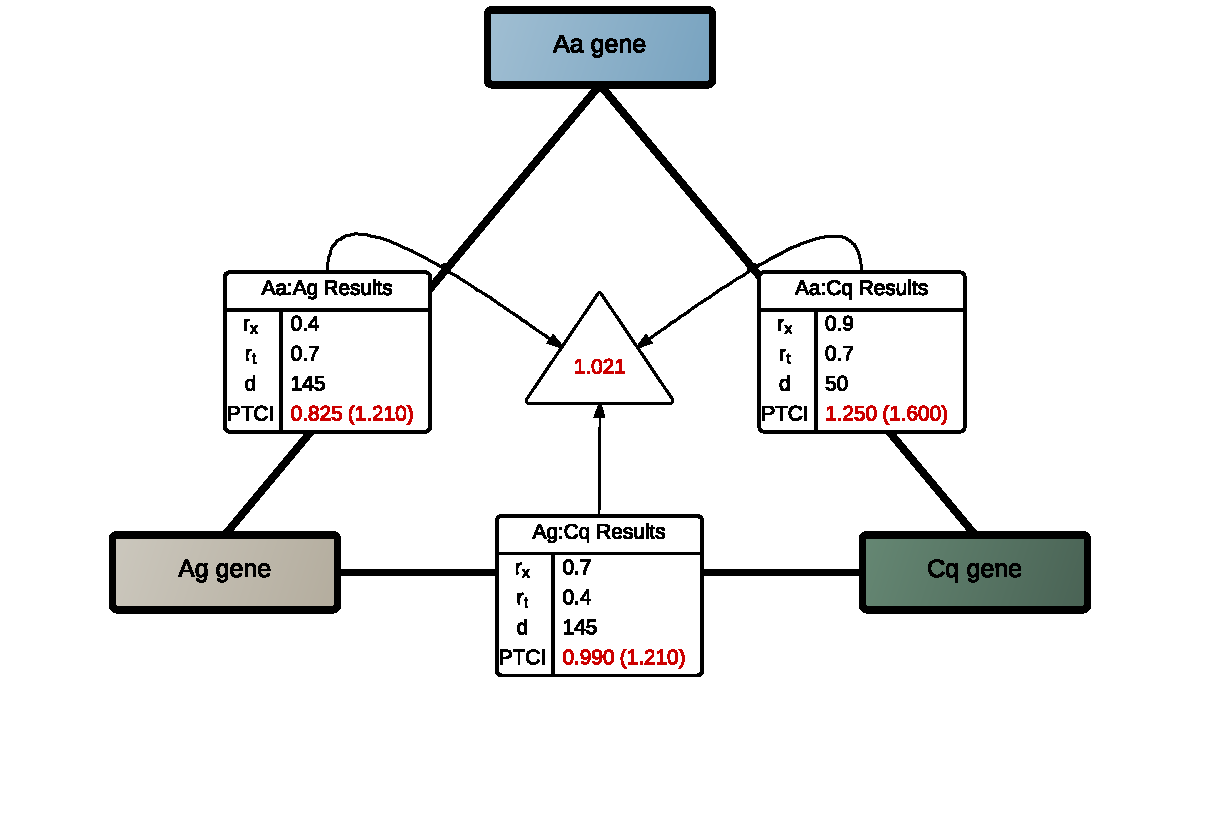
\includegraphics[width=\linewidth]{figures/figs/gfunc_graph_figs/ortho-graph-ptci.pdf}
    \caption{Example PTCI data}\label{fig:nway-ortholog-graph-ptci}
    \end{subfigure}
% 
% 
% 
\caption[Graph model used to integrate data types]{\sf \textbf{Graph model used to integrate data types.}}\label{fig:nway-ortholog-graph}
\end{figure}



\section{Custom Software Solutions}

Two core bodies of software were developed for this project as well as numerous smaller custom Python scripts.
Blacktie is a python package that automates data flow between and record keeping for analysis runs of the components of the third-party analysis pipeline dubbed the \gls{TuxProt} \cite{Trapnell2012}.
The purpose of the second software project, the \gls{gFunc}, is to provide a framework with which to integrate many, disparate data types to facilitate the synthesis of functional genomics analyses that make use of as many types of data as may be useful.

Blacktie's code and documentation have been made available to the public.
It is hosted as a \gls{Git} project with the complete history of code commits included and available for easy open source improvement and collaboration.
It is also available as an easily installable package from the \gls{PyPI} for general users.
It has been downloaded and installed over 2000 times as of this time with its latest version (v0.2.1.2) being downloaded at least 327 times (according to \gls{PyPI}).

\gls{gFunc} is based around an existing, well known, and well maintained network-graph framework called networkx \cite{Hagberg2008}.
\gls{gFunc} uses this code library as a database backbone and provides a framework for installing common genomic data-types into the graph structure as well as a convention for extending the core objects of \gls{gFunc} to handle new types of data.
The project is not formally released.
After using it for my own work, I have learned more about how best to organize the code.
Once it has been re-factored to incorporate the lessons learned here (mainly that the core objects should be simplified as much as possible and more of the data management should be coded directly with networkx rather than re-implementing certain functions), it will be released to the public using the same mechanisms as described for Blacktie.


\subsection{Blacktie RNA-seq pipeline}

See Figure \ref{fig:tuxedo}




\begin{landscape}
 
 
 \begin{figure}[hp]
\centering
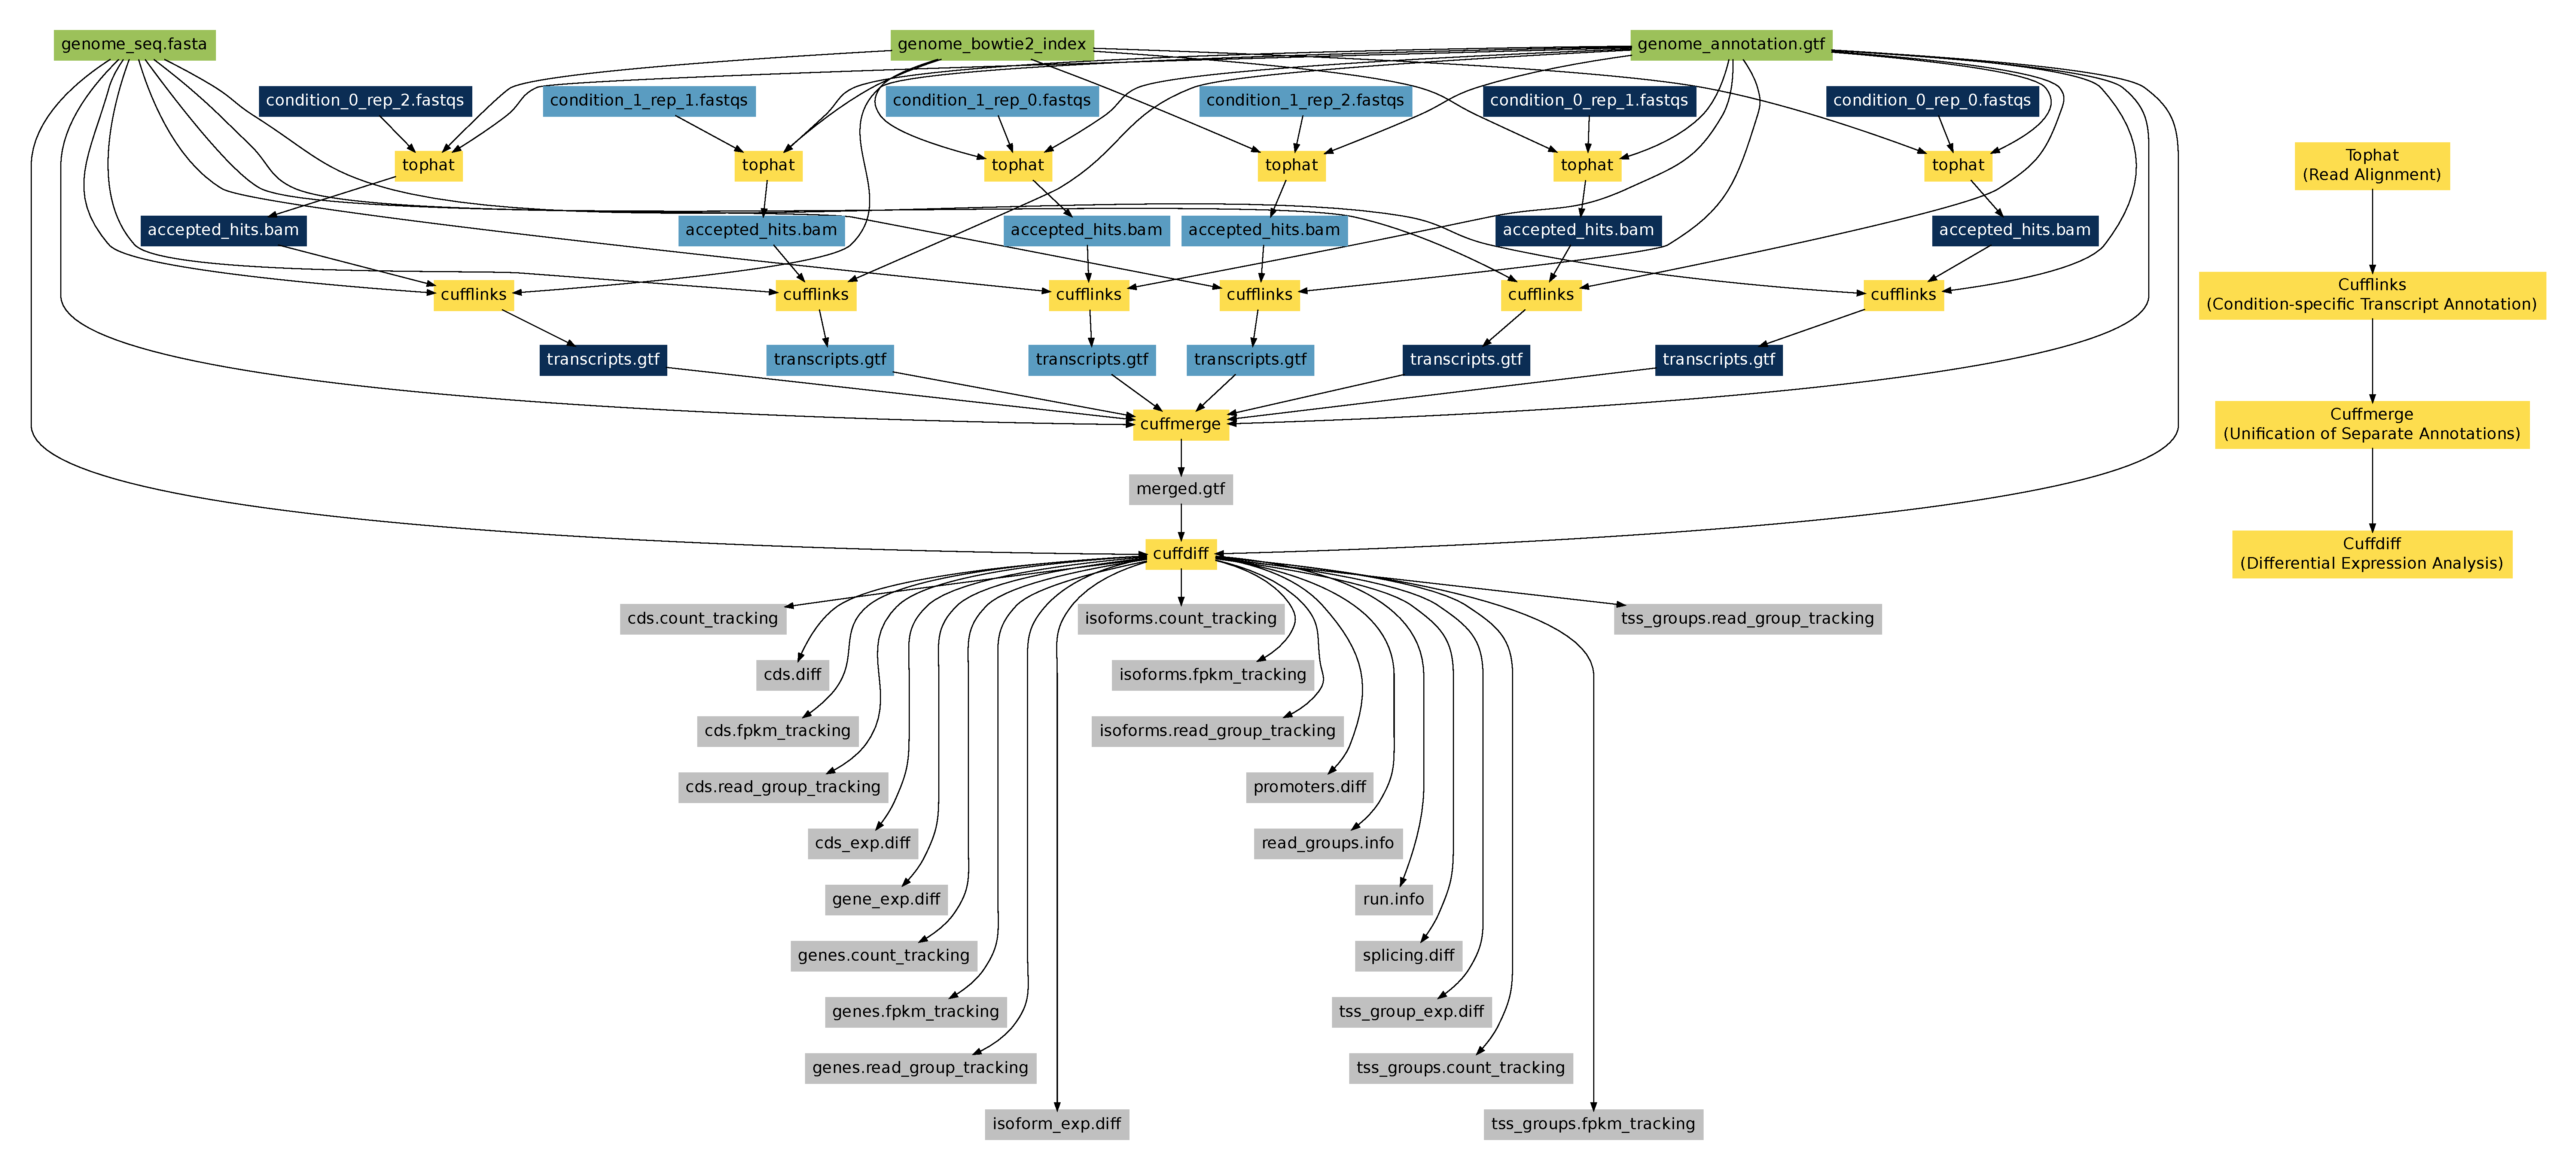
\includegraphics[width=\linewidth]{figures/figs/tuxedo_dot/707354_6/tophat_cufflinks_ins_outs.pdf}
\caption[Diagram of Abbreviated Tophat/Cufflinks Inputs and Outputs]{\sf \textbf{Diagram of Abbreviated Tophat/Cufflinks Inputs and Outputs:}\\
	This figure demonstrates the complexities of a typical RNA-seq experiment as analyzed with the \gls{TuxProt}. It models a fairly \textbf{simple} two condition experiment with each condition having three replications. It is ``abbreviated'' in that it only displays the output files that will be used in the next step for all steps except the \UseVerb{cuffdiff} step. The complete output of \UseVerb{cuffdiff} is included to demonstrate the final challenge of integrating the data which exists in multiple cross-referenced files.\\ 
	(\emph{Dark Blue} - Inputs/Outputs associated with Condition Zero; 
	\emph{Light Blue} - Inputs/Outputs associated with Condition One; 
	\emph{Grey} - Inputs/Outputs associated with Condition Zero \textbf{AND} Condition One; 
	\emph{Green} - Inputs Specific to the Reference Genome; 
	\emph{Gold} - Program Calls)
}
	\label{fig:tuxedo}
\end{figure}
 
 
 
\end{landscape}






%%% Local Variables: ***
%%% mode: latex ***
%%% TeX-master: "thesis.tex" ***
%%% End: ***
